\documentclass[a4paper]{oblivoir}
\usepackage{amsmath,amssymb,kotex,kswrapfig,mdframed,paralist}
\usepackage{fapapersize}
\usefapapersize{210mm,297mm,20mm,*,20mm,*}

\usepackage{tabto,pifont}
\TabPositions{0.2\textwidth,0.4\textwidth,0.6\textwidth,0.8\textwidth}

%%% 객관식 선지
\newcommand\one{\ding{172}}
\newcommand\two{\ding{173}}
\newcommand\three{\ding{174}}
\newcommand\four{\ding{175}}
\newcommand\five{\ding{176}}
\usepackage{tabto,pifont}
%\TabPositions{0.2\textwidth,0.4\textwidth,0.6\textwidth,0.8\textwidth}

\newcommand\taba[5]{\par\noindent
\one\:{#1}
\tabto{0.2\textwidth}\two\:\:{#2}
\tabto{0.4\textwidth}\three\:\:{#3}
\tabto{0.6\textwidth}\four\:\:{#4}
\tabto{0.8\textwidth}\five\:\:{#5}}

\newcommand\tabb[5]{\par\noindent
\one\:{#1}
\tabto{0.33\textwidth}\two\:\:{#2}
\tabto{0.67\textwidth}\three\:\:{#3}\medskip\par\noindent
\four\:\:{#4}
\tabto{0.33\textwidth}\five\:\:{#5}}

\newcommand\tabc[5]{\par\noindent
\one\:{#1}
\tabto{0.5\textwidth}\two\:\:{#2}\medskip\par\noindent
\three\:\:{#3}
\tabto{0.5\textwidth}\four\:\:{#4}\medskip\par\noindent
\five\:\:{#5}}

\newcommand\tabd[5]{\par\noindent
\one\:{#1}\medskip\par\noindent
\two\:\:{#2}\medskip\par\noindent
\three\:\:{#3}\medskip\par\noindent
\four\:\:{#4}\medskip\par\noindent
\five\:\:{#5}}

\usepackage{graphicx}

%\pagestyle{empty}

%%% Counters
\newcounter{num}

%%% Commands
\newcommand{\prob}[1]
{\bigskip\bigskip\noindent\refstepcounter{num}\textbf{문제 \arabic{num})} #1\par\noindent}


\newcommand\pb[1]{\ensuremath{\fbox{\phantom{#1}}}}

\newcommand\ba{\ensuremath{\:|\:}}

\newcommand\vs[1]{\vspace{40pt}}

\newcommand\an[1]{\bigskip\par\noindent\textbf{문제 #1)}\par\noindent}

%%% Meta Commands
\let\oldsection\section
\renewcommand\section{\clearpage\oldsection}

\let\emph\textsf

\begin{document}
\begin{center}
\LARGE태희, 미니테스트 01
\end{center}
\begin{flushright}
날짜 : 2018년 \(\pb3\)월 \(\pb{10}\)일 \(\pb{월}\)요일
,\qquad
제한시간 : \pb{17년}분
,\qquad
점수 : \pb{20} / \pb{20}
\end{flushright}

%
\prob{}
12명으로 구성되어 있는 동아리에서 회장, 부회장, 총무를 각각 1명씩 선출하는 방법의 수는?
\taba{780}{850}{870}{980}{1320}

%
\prob{}
등식 \(_n\text P_2+4_n\text P_1=28\)을 만족시키는 \(n\)의 값은?
\taba34567

%
\prob{}
6개의 문자 \(a\), \(b\), \(c\), \(d\), \(e\), \(f\)를 일렬로 배열할 때, \(a\), \(f\)가 이웃하는 경우의 수를 구하여라.

%
\prob{}
남학생 4명과 여학생 3명이 일렬로 나열된 7개의 의자에 앉는다.
이때, 여학생끼리 이웃하지 않도록 앉는 방븝의 수를 구하여라.

%
\prob{}
picture의 7개 문자를 일렬로 나열할 때, 적어도 한쪽 끝에 모음이 오는 경우의 수는?
\taba{3560}{3600}{3640}{3680}{3720}

%
\prob{}
0, 1, 2, 3, 4, 5의 6개의 숫자를 한 번씩만 사용하여 만들 수 있는 세 자리의 자연수 중 적어도 한쪽 끝이 짝수인 자연수의 개수는?
\taba{68}{72}{76}{80}{84}

%
\prob{}
두 집합 \(X=\{1,2,3\}\), \(Y=\{a,b,c,d,e\}\)에 대하여 \(X\)에서 \(Y\)로의 함수의 개수를 \(x\), 일대일 함수의 개수를 \(y\)라고 할 때, \(x+y\)의 값은?
\taba{160}{185}{200}{235}{250}

\newpage
%
\prob{}
다음과 같은 도로망에서 \(A\)에서 \(P\)를 거쳐 \(B\)로 가는 최단 경로의 수는?
\begin{center}
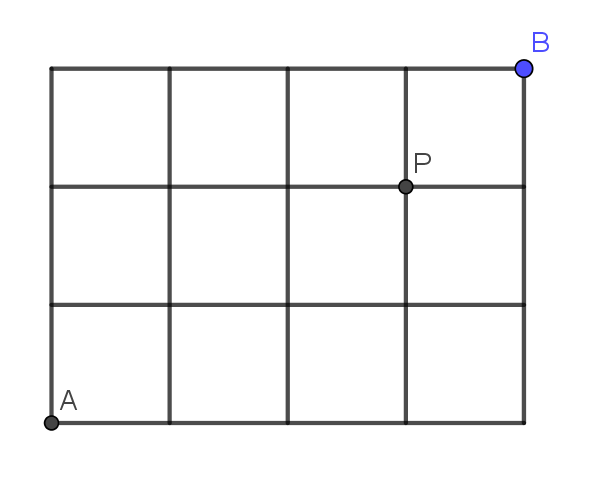
\includegraphics[width=0.3\textwidth]{route}
\end{center}
\taba8{12}{20}{48}{60}

%
\prob{}
\(_{12}C_{r-3}=_{12}C_{3r-1}\)을 만족시키는 \(r\)의 값은?

%
\prob{}
\(_5C_3=_nC3+_4C_2\)를 만족시키는 \(n\)의 값을 구하여라.

%
\prob{}
탁구 모임의 회원 10명 중 3명의 대표를 뽑는 방법의 수를 구하여라.

%
\prob{}
1, 2, 3, 4, 5, 6의 자연수가 하나씩 쓰여 있는 6장의 카드 중에서 2장의 카드를 뽑을 때, 짝수가 쓰여 있는 카드를 적어도 1장 뽑는 경우의 수를 구하여라.

%
\prob{}
5개의 과일과 3개의 야채 중에서 3개의 과일과 2개의 야채를 택하여 일렬로 나열하는 방법의 수는?
\taba{1200}{2400}{3600}{4800}{6000}
\end{document}